
\begin{definition} [Conjunto de nivel] 
\label{def:conjunto de nivel}
 \mbox{}
 
Sea $f: U\subset\Rn{n}\rightarrow\R$ y sea $c \in \R$, se define  el conjunto de nivel de $f$ de nivel  $c$, y se nota $C(c,f)$,  a  
\[
C(c,f)=\{ x \in U \backslash f (x)=c \}.
 \]





Es decir,  $C(c,f)$ son aquellos puntos $x\in\ U$ para las cuales $f(x)=c$, o dicho de otra manera,  $C(c,f)$ es la preimagen de $c$ por $f$.   Si $n=2$ hablamos de curva de nivel  y si $n=3$  hablamos de superficie de nivel  

Observaci\'on: \textcolor{red}{Enumerar}   Si $f: A\subseteq\Rn{n}\rightarrow\R$ entonces $C(c,f)  \subset \mathbb{R}^{n}.$



\begin{example}   Sea  el campo  $f: \mathbb{R}^{2} \rightarrow \mathbb{R} \:|\:  f(x,y)=x^2+y^2.$
\end{example}
1. Calcular y graficar los conjuntos de nivel de $f$.

2. Hacer un gr\'afico de  $graf(f)$.



Observemos que, dado $c \in \mathbb{R}$: 
 $$C(c,f)=\{(x,y) \in U \backslash   x^2+y^2  =c \}.$$
 Tomando, para ilustrar,  $c=0$, $c=1$ y $c=4$, quedando (ver (\ref{circ})) 
 \[
C(0,f)=\{(x,y) \in U \backslash x^2+y^2=0 \}
\]
 \[
C(1,f)=\{(x,y) \in U \backslash x^2+y^2=1 \}
\]
 \[
C(4,f)=\{(x,y) \in U \backslash x^2+y^2=4 \}
 \]

\begin{figure}[h!] % El entorno figure te permite incluir imágenes
    \centering
    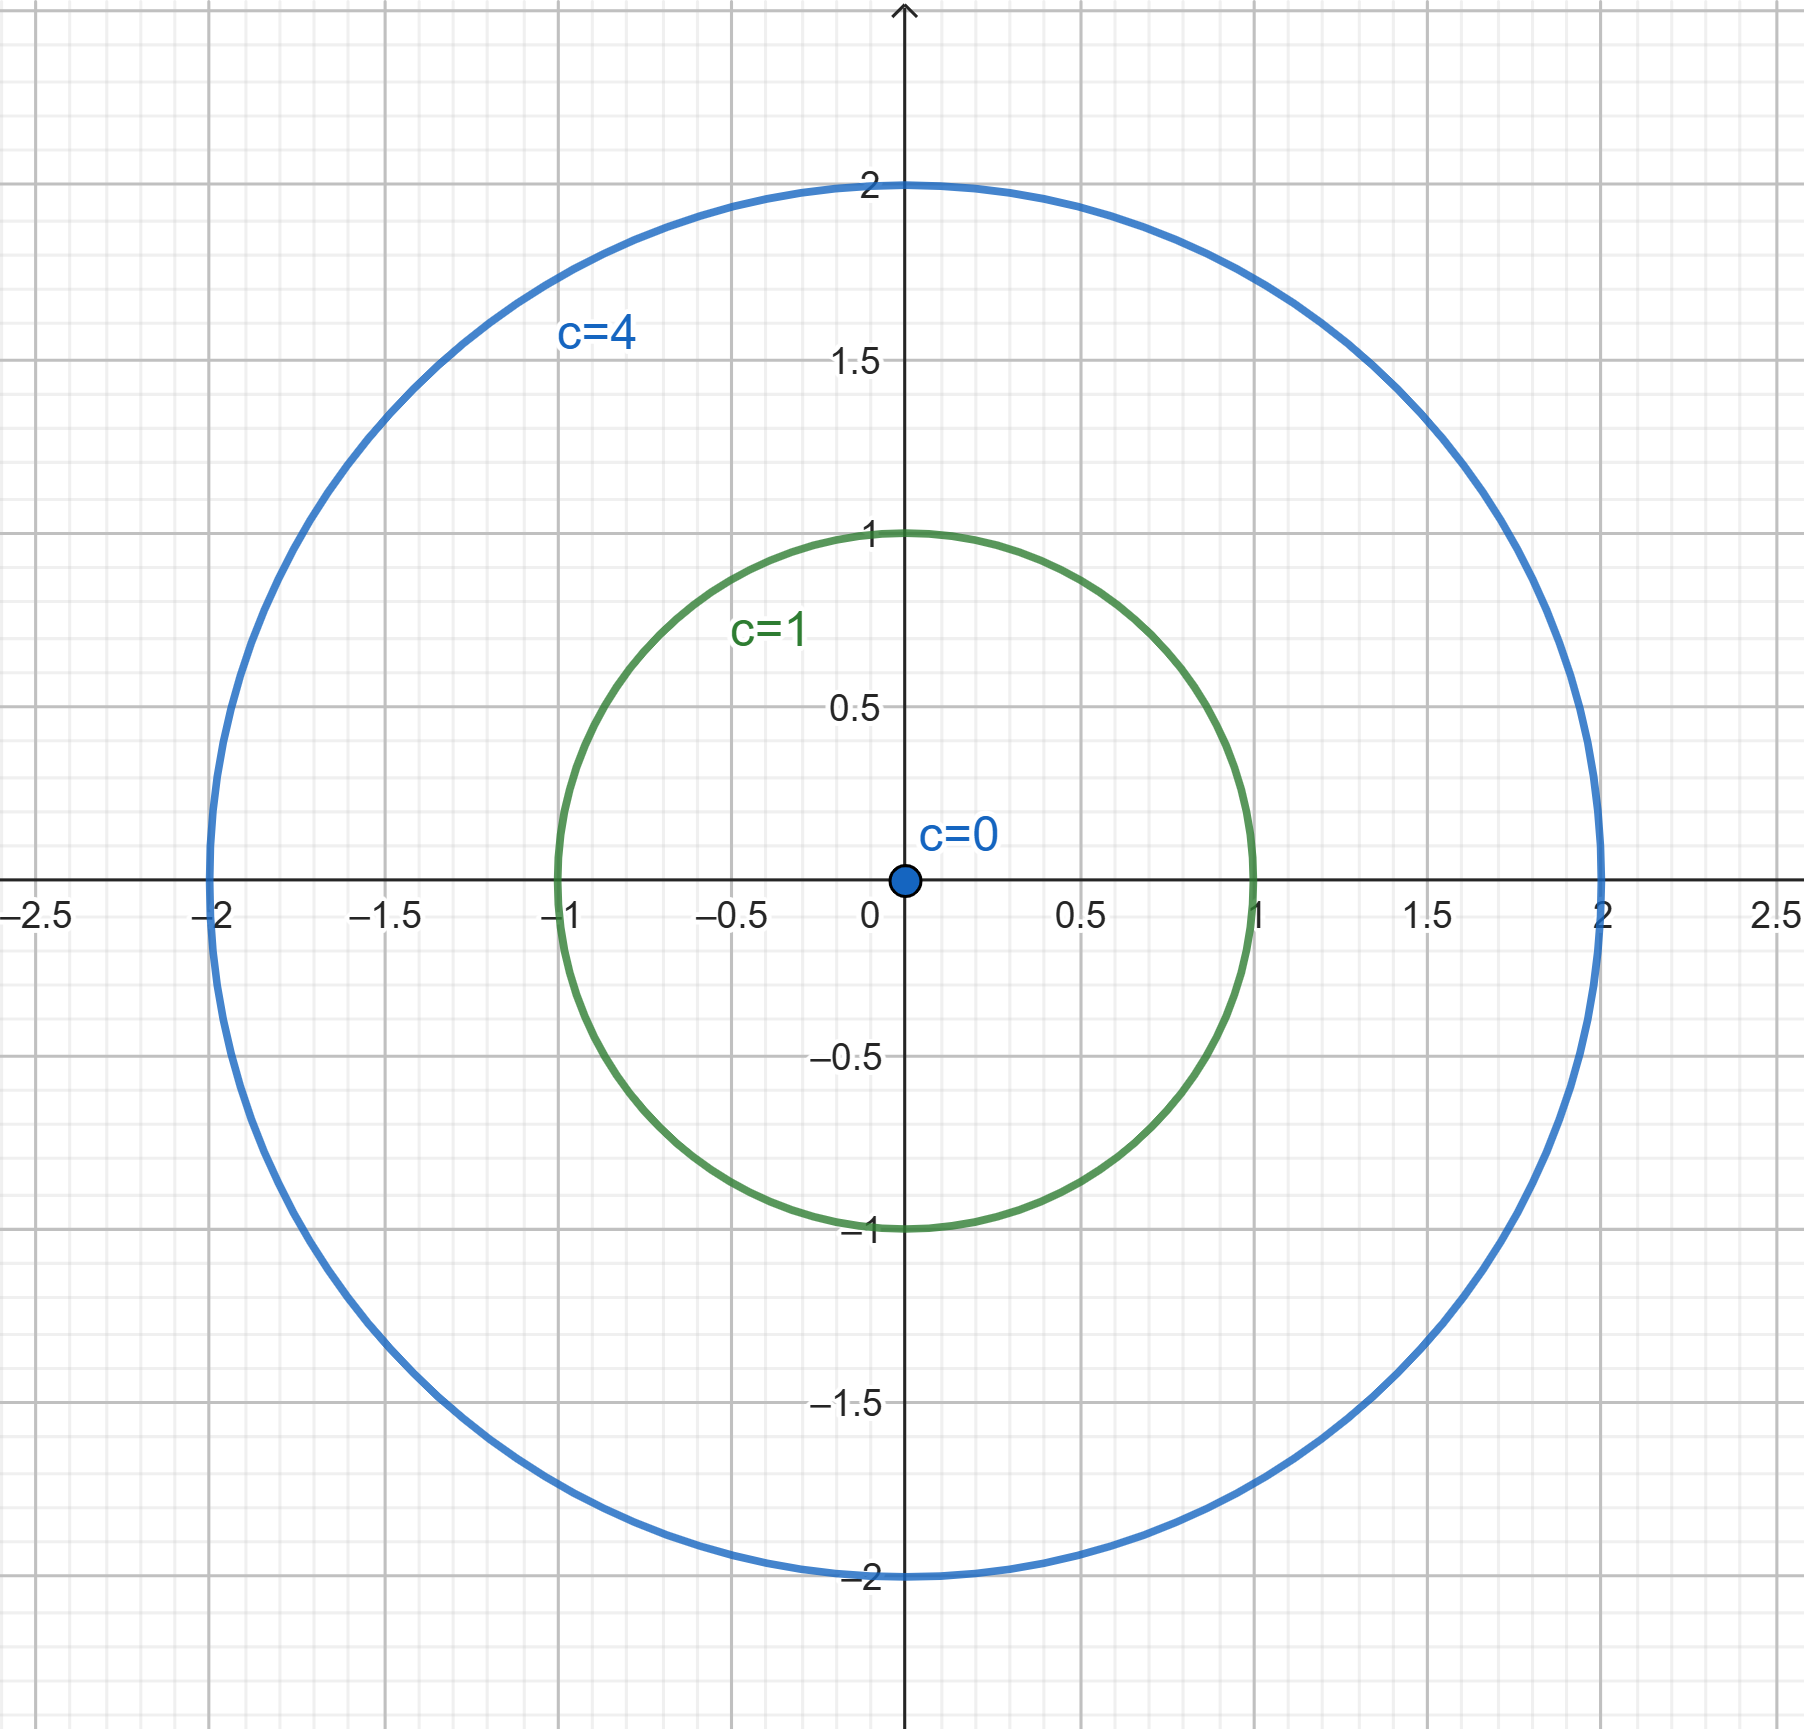
\includegraphics[width=0.5\textwidth]{../figs/conjunto1_r.png} % Cambia esta ruta por la ubicación de tu imagen
    \caption{Conjuntos de nivel}
    \label{fig:ejemplo} % Etiqueta para hacer referencia a la imagen
\end{figure}

En general, podemos determinar: 

   \[
        C(c,f)=
        \begin{dcases}
           \textnormal{Circunferencia centrada en (0,0) de radio} \sqrt{c},  & \textnormal{si}:  c>0 \\
(0,0)  & \textnormal{si}:\ c=0\\
\emptyset  & \textnormal{si}:\ c<0\\
        \end{dcases}
    \]

\textcolor{red}{Aca ``dibujar'' los conjuntos de nivel en $\mathbb{R}^{3}$ y notar que no es suficinte para graficar.}  


\textcolor{red}{Definir cortes transversales y dibujarlos.}


\begin{figure}[h!] % El entorno figure te permite incluir imágenes
    \centering
    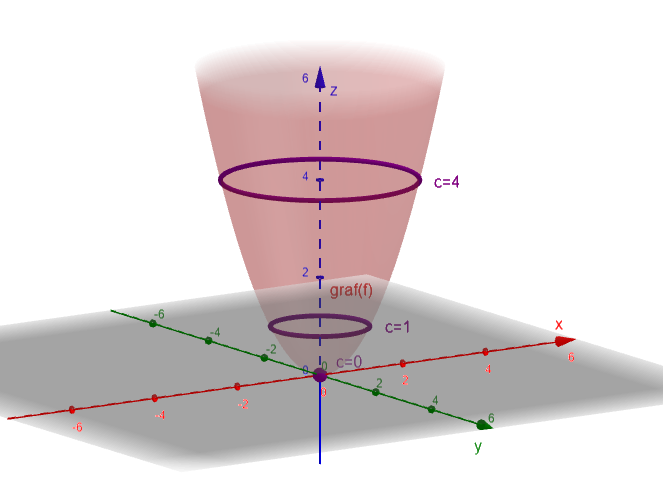
\includegraphics[width=0.5\textwidth]{../figs/conjunto1_r3.png} % Cambia esta ruta por la ubicación de tu imagen
    \caption{graf(f)}
    \label{fig:ejemplo} % Etiqueta para hacer referencia a la imagen
\end{figure}



 

\begin{example}   Sea  el campo  $g: \mathbb{R}^{2} \rightarrow \mathbb{R} \:|\:  g(x,y) = \sqrt{x^2+y^2}.$
\end{example}
1. Calcular y graficar los conjuntos de nivel de $g$.

2. Hacer un gr\'afico de  $graf(g)$.


\textcolor{red}{Resolver identico al ejercicio  anterior.}  



: Se toma la funcion $f(x,y)=\sqrt{x^2+y^2}$, donde empezamos a analizar los distintos conjuntos de nivel, tomando $c$ con diferentes constantes
 \[
C(0,f)=\{(x,y) \in U \backslash \sqrt{x^2+y^2}=0 \}
\]
 \[
C(1,f)=\{(x,y) \in U \backslash \sqrt{x^2+y^2}=1 \}
\]
 \[
C(2,f)=\{(x,y) \in U \backslash \sqrt{x^2+y^2}=2 \}
 \]

\begin{figure}[h!] % El entorno figure te permite incluir imágenes
    \centering
    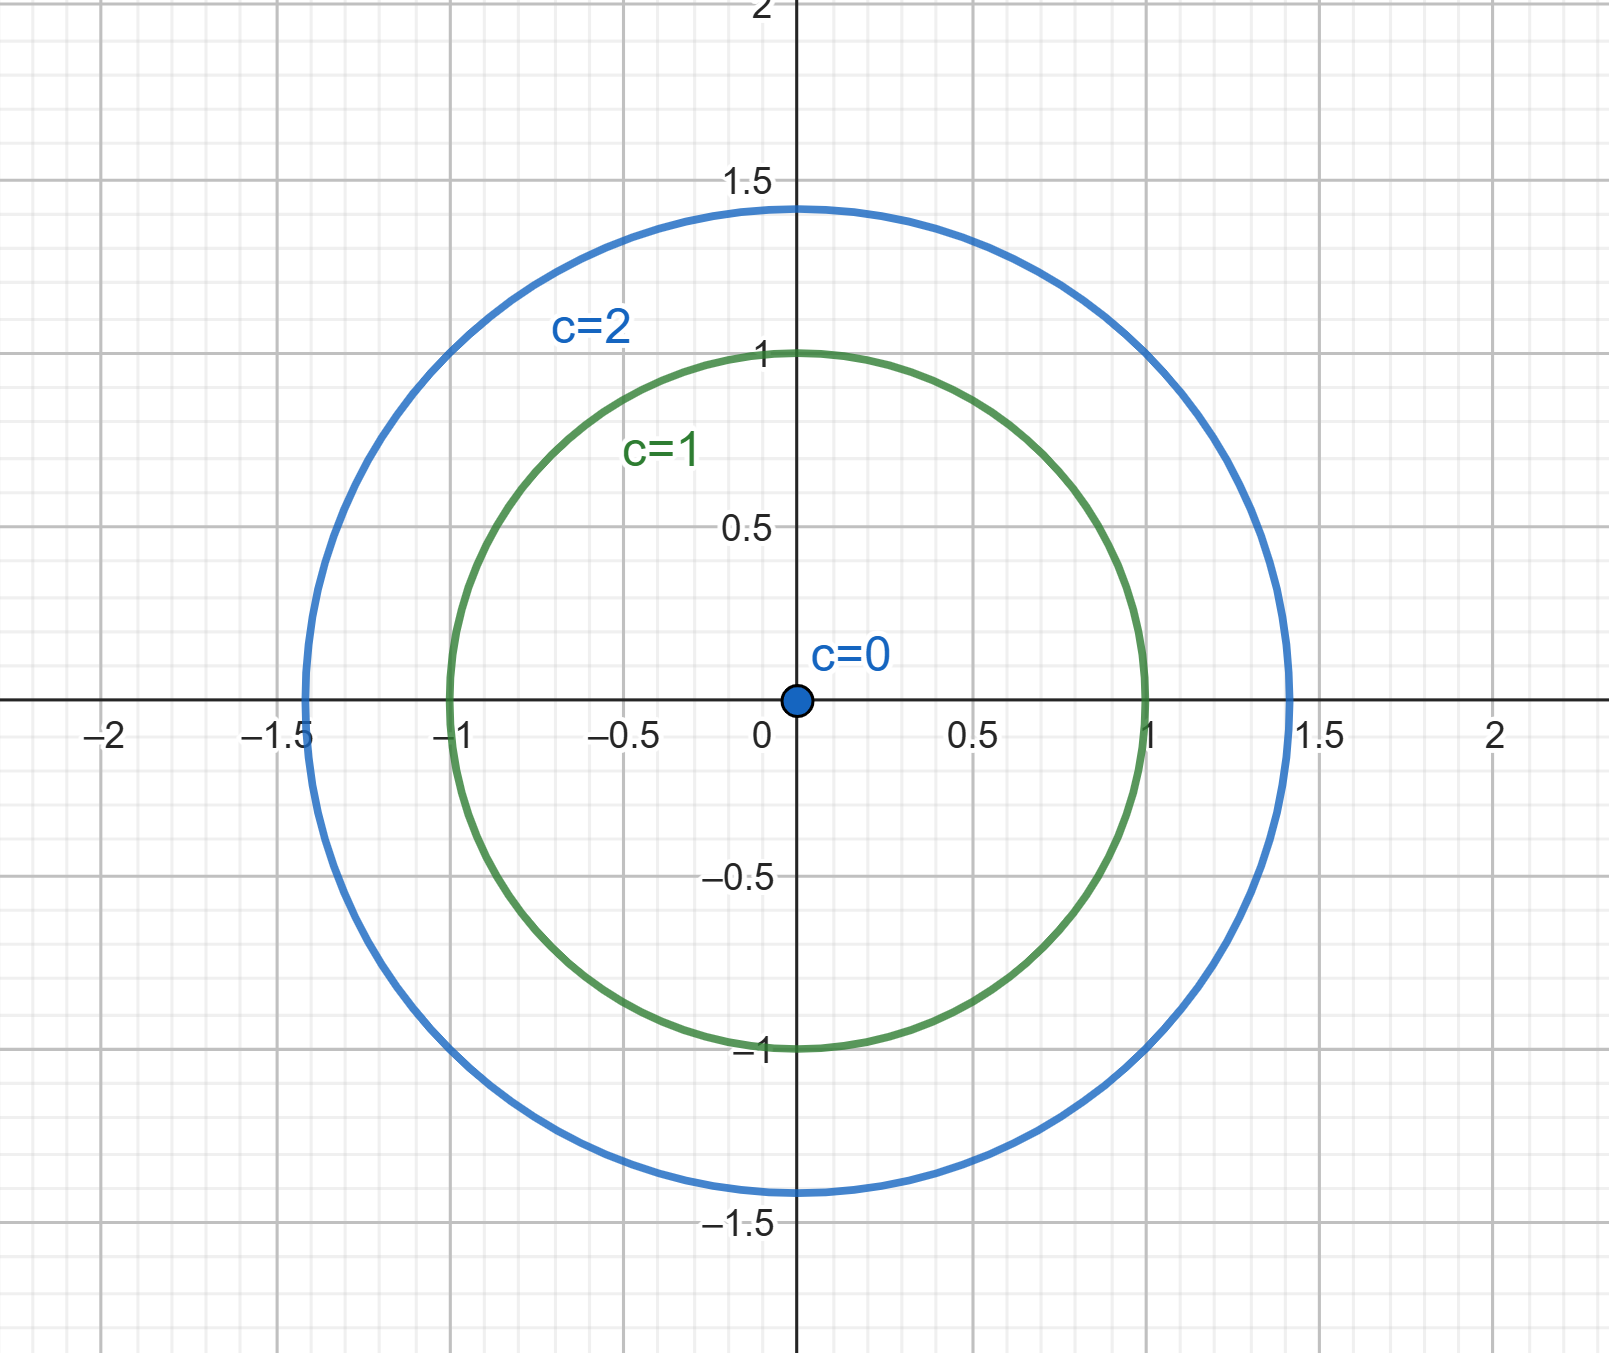
\includegraphics[width=0.5\textwidth]{../figs/conjunto2_r2.png} % Cambia esta ruta por la ubicación de tu imagen
    \caption{Conjuntos de nivel}
    \label{fig:ejemplo} % Etiqueta para hacer referencia a la imagen
\end{figure}

En general, podemos determinar: 

   \[
        C(c,f)=
        \begin{dcases}
           \textnormal{Circunferencia centrada en (0,0) de radio} c,  & \textnormal{si}:  c>0 \\
(0,0)  & \textnormal{si}:\ c=0\\
\emptyset  & \textnormal{si}:\ c<0\\
        \end{dcases}
    \]
\begin{figure}[h!] % El entorno figure te permite incluir imágenes
    \centering
    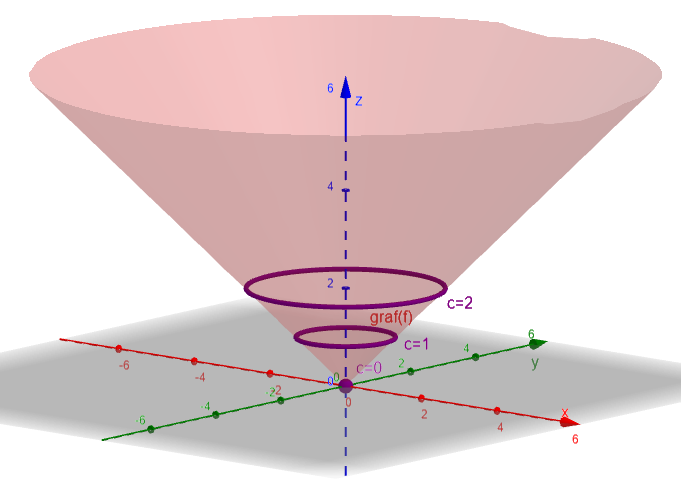
\includegraphics[width=0.5\textwidth]{../figs/conjunto2_r3.png} % Cambia esta ruta por la ubicación de tu imagen
    \caption{Conjuntos de nivel y graf(f)}
    \label{fig:ejemplo} % Etiqueta para hacer referencia a la imagen
\end{figure}

De esta manera, considerando la definicion de gráfica de una funci\'on, podemos representar la misma en $\Rn{3}$ tomando  la ecuaci\'on de la parte superior de un cono: $z=\sqrt{x^2+y^2}$



\textcolor{red}{Corregir esta observaci\'on. esta mal escrito, quien es la funci\'on f?}


Observaci\'on \textcolor{red}{enumerar}:Dada la  ecuaci\'on $z^2=x^2+y^2$ al despejar z obtenemos $|z|=\sqrt{x^2+y^2}$ obtendriamos que: 
 \[
        C(c,f)=
        \begin{dcases}
           \textnormal{Circunferencia centrada en (0,0) de radio} c,  & \textnormal{si}:  c>0 \\
(0,0)  & \textnormal{si}:\ c=0\\
\textnormal{Circunferencia centrada en (0,0) de radio} c,  & \textnormal{si}:\ c<0\\
        \end{dcases}
    \]

De esta manera, considerando la definicion de gráfica de una funcion, podemos representar la misma en $\Rn{3}$ tomando  la ecuacion del cono: $z^2=x^2+y^2$

\begin{figure}[h!] % El entorno figure te permite incluir imágenes
    \centering
    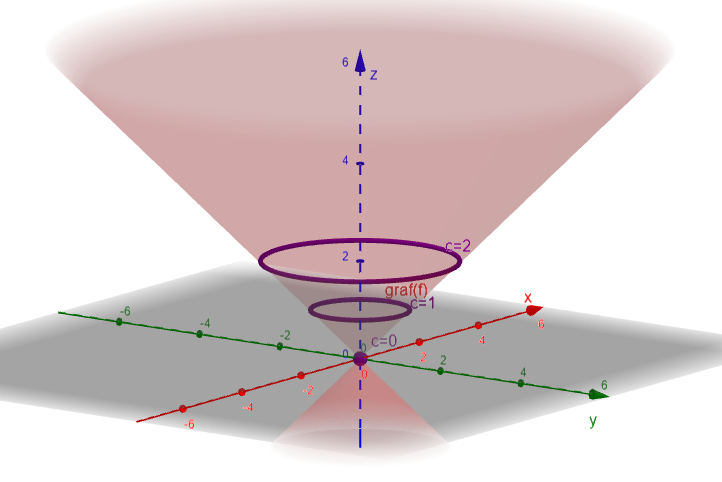
\includegraphics[width=0.5\textwidth]{../figs/conjunto3_r3.png} % Cambia esta ruta por la ubicación de tu imagen
    \caption{Conjuntos de nivel y graf(f)}
    \label{fig:ejemplo} % Etiqueta para hacer referencia a la imagen
\end{figure}


\textcolor{red}{Mejorar la figura, no se llega a apreciar el cono completo}

\end{definition}
